\begin{figure}[h] 
\centering 
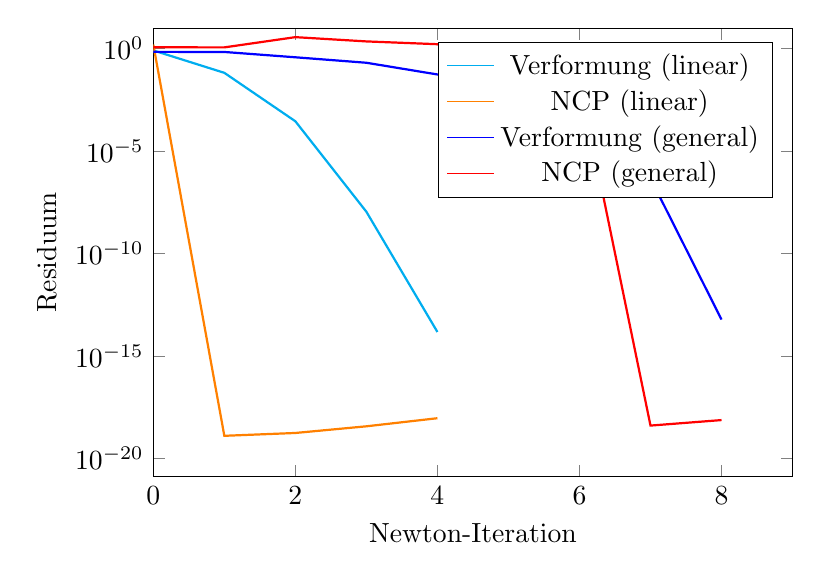
\begin{tikzpicture}[every plot/.append style={thick}] 
\begin{axis}[ 
label style={font=\normalsize}, 
xlabel={Newton-Iteration}, 
ylabel={Residuum}, 
xmin=0, xmax=9, 
ymode=log, 
ymin=0, ymax=10, 
width=0.8\textwidth, 
height=0.6\textwidth, 
legend pos=north east, 
legend style={cells={align=left}}, 
grid style=dashed, 
] 
\addplot[ 
color=cyan, 
] 
coordinates { 
(0, 8.23e-01)(1, 6.64e-02)(2, 2.86e-04)(3, 1.09e-08)(4, 1.47e-14)}; 
\addlegendentry{Verformung (linear)} 
\addplot[ 
color=orange, 
] 
coordinates { 
(0, 1.60e+00)(1, 1.25e-19)(2, 1.72e-19)(3, 3.64e-19)(4, 9.05e-19)}; 
\addlegendentry{NCP (linear)} 
\addplot[ 
color=blue, 
] 
coordinates { 
(0, 7.02e-01)(1, 6.93e-01)(2, 3.81e-01)(3, 2.06e-01)(4, 5.52e-02)(5, 2.64e-02)(6, 1.66e-03)(7, 4.62e-07)(8, 5.93e-14)}; 
\addlegendentry{Verformung (general)} 
\addplot[ 
color=red, 
] 
coordinates { 
(0, 1.17e+00)(1, 1.16e+00)(2, 3.67e+00)(3, 2.27e+00)(4, 1.66e+00)(5, 3.11e-02)(6, 2.74e-02)(7, 3.95e-19)(8, 7.34e-19)}; 
\addlegendentry{NCP (general)} 
\end{axis} 
\end{tikzpicture} 
\caption{Residuen des Stoffgesetzes 'Neo Hooke' mit Hinderniss 'Hut' und 2178 Freiheitsgraden für die Verschiebung.} 
\label{fiq:NeoHooke_Hut_level4} 
\end{figure} 
